\section{The Extensible Compiler}\label{sec:compiler}

In order to realize the CMP \cite{cmp} manifesto's vision,
the CML compiler generates code in any target language based on extensible templates.
A set of core templates is provided by the CML compiler's base libraries.
Third-party libraries can also provide their own templates,
along with their conceptual models,
in order to target specific technologies or platforms.
Developers can also extend existing templates in order to adapt the implementation to characteristics specific to their projects.

Subsection \ref{subsec:overview} will provide an overview of the CML compiler's architecture.
Next, subsection \ref{subsec:templates} will introduce the CML compiler's extensible templates.
Finally, subsection \ref{subsec:modlib} will lay out the CML compiler's mechanism for organizing and sharing conceptual models and extensible templates.

\subsection{Compiler Overview}\label{subsec:overview}

An overview of the CML compiler's architecture is shown in figure \ref{fig:overview}.

\begin{figure}
\centering
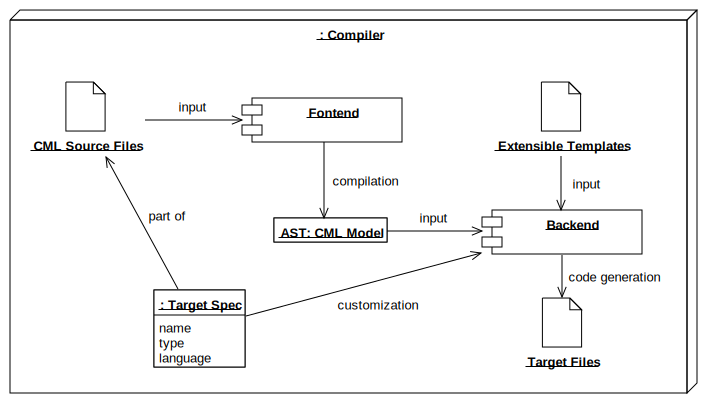
\includegraphics[width=\textwidth]{compiler/figure-overview}
\caption{An architectural overview of the CML compiler.}
\label{fig:overview}
\end{figure}

\subsection{Extensible Templates}\label{subsec:templates}

Terence Parr has formalized and developed the StringTemplate \cite{st} language for code generation. CML extensible templates are implemented in StringTemplate. The CML compiler uses StringTemplate for two purposes:

\begin{itemize}
\item \emph{file names and directory structure:}
each type of target generated by the CML compiler requires a different directory structure.
The CML compiler expects each target type to define a template file named ``files.stg'' (also known as \emph{files template}),
which will contain the path of all files to be generated. The \emph{files template} may use information provided by the \emph{target specification} (introduced in subsection \ref{subsec:overview}) in order to determine the file/directory names. Figure X shows an example of a \emph{files template}.
\item \emph{file content generation:}
each file listed under the \emph{files template} will have a corresponding \emph{content template} that specifies how the file's content must be generated. The \emph{content template} will receive as input one root-level element of the CML model, which will provide information to generate the file's content. The type of model element received as input by the \emph{content template} depends on which function of the \emph{files template} has defined the file to be generated. Figure Y shows a typical \emph{content template}. 
\end{itemize}

For example, ...

\subsection{Modules and Libraries}\label{subsec:modlib}

TODO: Check .NET assembly specification.

TODO: Check Java module specification.

When developing a single application with just a few targets, having a single directory to maintain all the source code is sufficient. But once one needs to develop more than one application (as part of a larger project) and share code among them, it is necessary to separate the common code. Also, some applications cover different domains, and it may be beneficial to separate the code into different CML models.

In order to allow that, CML supports \emph{modules}. Grouping a set of elements of a CML model, a module in CML is conceptually similar to a UML \cite{uml} package. Physically, each module is a directory containing three sub-directories:

\begin{itemize}
\item \emph{source}: where the CML source files reside.
\item \emph{templates}: optional directory containing templates for code generation.
\item \emph{targets}: created by the CML compiler to contain each target sub-directory, which in turn contains the target files generated for a given target.
\end{itemize}

Under the \emph{source} directory, the module will be defined by a \emph{module specification}. If a module needs to reference CML model elements in other modules, then an import statement should define the name of the other modules. The compiler will then compile the imported modules before compiling the current module.

In order for the compiler to find the other modules, they must be in a directory with the module's name in the same directory where the current module is placed.

CML modules have no versions as they are maintained in the same code repository with the other modules they import. However, one can package a module as a library, which will have a version and the same name as the module. This library in turn can be published into a public (or company-wide) \emph{library site} in order to be shared with other developers.

A CML library is just a packaged, read-only module with a version of the format: 

\verbatimfont{\small}
\begin{verbatim}
revision[.accretion][.fix]
\end{verbatim}

TODO: check semantic versioning

Where:
\begin{itemize}
\item \emph{revision} is the number of a library release incompatible with any previous releases with a lower revision number.
\item \emph{accretion} is the number of a library release compatible with any previous accretion number of the same revision.
\item \emph{fix} is the number of a library release that fixes an issue in a previous accretion.
\end{itemize}

Compatible versions do not change or remove public elements of the library's CML model (or function/parameters from the library's templates) but only add new elements. Fixes cannot change the library's public elements; only internal elements. These rules may be enforced by the CML compiler when packaging and publishing new versions of a library.

